\documentclass{article}
\usepackage[utf8]{inputenc}
\usepackage[a4paper, total={6.5in, 9.5in}]{geometry}
\usepackage[bookmarks,hidelinks]{hyperref}
\usepackage{amsmath, amssymb, dsfont}
\usepackage{mathtools}
\usepackage{chemfig}
\usepackage{chemformula}
\usepackage{xcolor}
\definecolor{gray07}{gray}{0.7}
\usepackage{float}
\usepackage{enumitem}
\usepackage{cancel}
\usepackage{pgfplots}
\usepgfplotslibrary{units} % to add units easily to axis
\usepgfplotslibrary{fillbetween} % to fill inbetween curves
\usepgfplotslibrary{colormaps} % to create colormaps
\pgfplotsset{width=12.2cm, height=7cm}
\pgfplotsset{compat=newest} %(making it only compatalbe with
%new releases of pgfplots)
\pgfdeclarehorizontalshading{visiblelight}{50bp}{
color(0.00000000000000bp)=(violet);
color(8.33333333333333bp)=(blue);
color(16.66666666666670bp)=(cyan);
color(25.00000000000000bp)=(green);
color(33.33333333333330bp)=(yellow);
color(41.66666666666670bp)=(orange);
color(50.00000000000000bp)=(red)
}%
\usepackage{tikz}
\usetikzlibrary{decorations.pathreplacing}
\usepackage{multirow}
\usepackage{caption}
\usepackage[load-configurations = abbreviations]{siunitx}
\sisetup{inter-unit-product=\ensuremath{{}\cdot{}}, exponent-product=\ensuremath{{}\cdot{}}, group-minimum-digits=3, range-phrase=-, range-units=single}
\usepackage{graphicx}
\graphicspath{ {./} }
\usetikzlibrary{shapes.arrows}
\let\ce\ch
\newcommand{\bit}{\text{bit}}
\newcommand{\equilibrium}[2]{$\ce{#1}\rightleftharpoons\ce{#2}$}
\newcommand{\soom}{\stackrel{10}{=}}
\newcommand{\vect}{\overrightarrow}
\newcommand{\formulaPyramidFactory}[4]{
    \begin{tikzpicture}[scale=1.25]
\draw (0,0) -- (-0.5, -0.75) node  [align=center, fill=white, midway] {\footnotesize \---};
\draw (0,0) -- (0.5, -0.75) node [align=center, fill=white, midway] {\footnotesize \---};
\draw (0.5, -0.75) -- (-0.5, -0.75) node [align=center, fill=white, midway] {\footnotesize #4};

\draw (0,0) node [above, fill=white] {#1};
\draw (-0.5, -0.75) node [left, fill=white] {#2};
\draw (0.5, -0.75) node [right, fill=white] {#3};

%\draw (0, -1) node [below, align=center] {\small (Pyramide de formule)};
\end{tikzpicture}
}
\newcommand{\formulaPyramid}[3]{\formulaPyramidFactory{#1}{#2}{#3}{$\times$}}
\newcommand{\formulaPyramidAdditive}[3]{\formulaPyramidFactory{#1}{#2}{#3}{$+$}}
\newenvironment{definitions}{\begin{description}[leftmargin=!,labelwidth=\widthof{\bfseries Lorem ipsum dolor}]}{\end{description}}
\newcommand{\deftable}[2]{%
%\hline
\begin{table}[h]
    \centering
    \begin{tabular}{llp{100mm}}%
        %& unité/type & Explication \\ \hline
        #1
    \end{tabular}
    \label{tab:#2_units}
\end{table}%
}
\newcommand{\deftablevar}[3]{%
    $#1$ & $\si{#2}$ & #3 \\
}
\newcommand{\deftableobj}[3]{%
    $#1$ & \textit{#2} & #3 \\
}

\title{Semaine 11}
\date{2020-06-17}
\author{Ewen Le Bihan}

\begin{document}

\maketitle

\section{Exercice I}

\subsection{}
\[
	\ce{C_8H_8O_3}
\] 
\subsection{}
\begin{figure}[h]
	\centering
	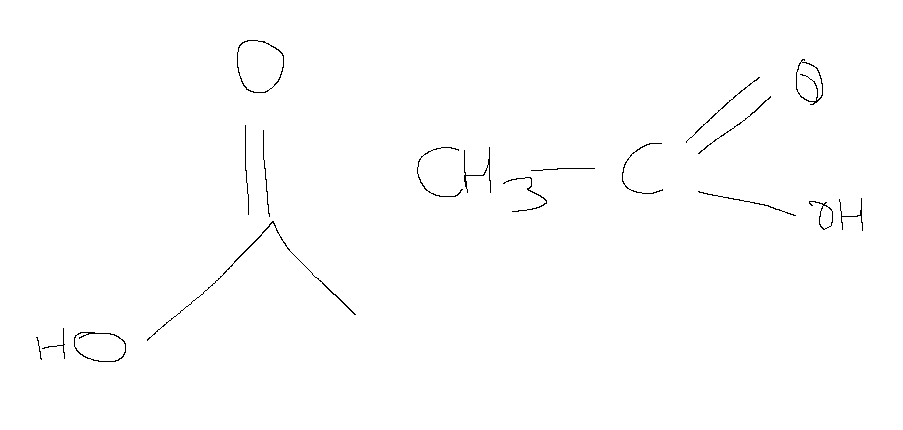
\includegraphics[width=0.8\textwidth]{./i-2.png}
	\caption{}
	\label{fig:}
\end{figure}
Acide éthanoïque

\subsection{}
\begin{description}
	\item[OH] Alcool
	\item[(en bas)] Aldéhyde
\end{description}

\subsection{}
\texttt{0 --[VanOH prédomine]-- pKa = 7.4 --[VanO- prédomine]-- 14}

\subsection{}
Hydroxhyde de sodium

\subsection{}

\begin{align*}
	\text{pH} &=  14 + \log C \\
	&= 13 \\
\end{align*}

\subsection{}
Ultraviolet

\subsection{}
Par construction graphique, la concentration $C$ est égale à $\SI{55}{\micro\mol\per\liter}$

\subsection{}
\begin{align*}
	m &= n \cdot M \\
	&= C \cdot V \cdot M \\
	&= 1 \cdot 100 \cdot 10^{-3} \cdot 152 \\
\end{align*}

\subsection{}
(non traité)

\section{Exercice III}

\subsection{}

\begin{align*}
	R_{\text{th}} &= \frac{L}{\lambda s} \\
	[R_{\text{th}}] &= \frac{[L]}{[\lambda][s]} \\
                 	&= \frac{\text{m}}{\text{W} \cancel{\text{m}^{-2}} \cdot \text{K}^{-1} \cdot \cancel{\text{m}^2}} \\
			&= \si{\kelvin\per\watt}  \\
\end{align*}

\subsection{$R_{\text{th}}$ totale (questions 2, 3, 4)}
\begin{align*}
	R_{\text{Total}} &= R_1 + R_2 + R_3 \\
	&= \frac{8 \cdot 10^{-2}}{0.15} + \frac{10 \cdot 10^{-2}}{0.042} + \frac{4 \cdot 10^{-2}}{0.16} \\
	&= \SI{3.2}{\kelvin\per\watt} \quad\text{pour 1 mètre carré} \\
	&=  3.2 \cdot \frac{1}{100}\\
	&= \SI{0.032}{\kelvin\per\watt} \\
\end{align*}

\begin{align*}
	\Phi &= \frac{\Delta T}{R_{\text{th}}} \\
          &= \frac{20 - (-10)}{0.032} \\
	  &\approx \SI{937.5}{\watt} \\
\end{align*}

\setcounter{subsection}{4}

\subsection{}

Il faut le moins de verre ($\lambda = 0.81$) et le plus d'argon possible ($\lambda = 0.018$):
\begin{description}
	\item[Moins isolant] (10-10-4) air
	\item[Plus isolant] (4-16-4) argon
\end{description}

\subsection{}

\begin{align*}
	P&= \frac{Q}{\Delta T} \\
	&= \frac{111 \cdot 10^{-6}}{3 \cdot 3600} \\
	&= \SI{10.2}{\kilo\watt} \\
\end{align*}

\subsection{}
\begin{align*}
	Q &= m \cdot c \cdot \Delta\Theta \\
\end{align*}

(skipped)

\setcounter{subsection}{8}

\subsection{}

\[
	\ce{C_3H_8+5O_2 -> 3CO_2+4H_2O}
\] 

\subsection{}

\begin{align*}
	m_{\ce{CO_2}} &= m \cdot M \\
	&= 210 \cdot 44 \\
	&= \SI{9}{\kilo\gram} \\
\end{align*}

\newpage\section{Modèle orbitalaire}


\end{document}
